% 원본 양식 출처 : http://forcecore.tistory.com/1113
\documentclass{beamer}
\usetheme{Singapore}

\usecolortheme{lily}

\usepackage{xcolor}
\usepackage[hangul]{kotex}%to input Korean letters
\usepackage{fancyvrb}%fancy verbatim
\usepackage{color}%to use color presets
\usepackage{graphicx}%includegraphics
\usepackage{epstopdf}%enables to include eps by converting to pdf
\usepackage{verbatim}%comment
\usepackage{comment}
\usepackage{gensymb}%\deg
\usepackage{listings}
\renewenvironment{comment}{}{}%http://tex.stackexchange.com/questions/45617/comment-package-not-working



\setbeamertemplate{blocks}[rounded][shadow=true]
\definecolor{blue1}{RGB}{0,0,80}
\definecolor{blue2}{RGB}{223, 223, 255}
\setbeamercolor{block title}{bg=blue1,fg=white}
\setbeamercolor{block body}{bg=blue2,fg=black}

\setbeamertemplate{navigation symbols}{}%to suppress navigation tools
\setbeamertemplate{footline}[text line]{%
	\parbox{\linewidth}{\vspace*{-8pt}경기과학고등학교 나는코더다 2016 송년 대회\hfill\hfill\insertpagenumber}}%footer

\begin{document}
	
	% title slide
	\begin{frame}
		\title{나는코더다 2016 송년 대회: Solution sketch}
		\author{14004 구재현 (koosaga)\newline 경기과학고등학교}
		\date{}
		\titlepage
	\end{frame}
	
	% outline slide
	%\section*{목차}
	%\begin{frame}
	%	\setcounter{tocdepth}{1}
	%	\tableofcontents
	%\end{frame}
	\begin{frame}
		\frametitle{도와주신 분들}
		\begin{itemize}
			\item GSHS TeX Society의 자료들이 모든 조판을 \LaTeX 로 진행하는 데 큰 도움이 되었습니다. 운영해주신 학우 분들께 감사드립니다.
			\item 대회 진행에 아낌없는 지원을 약속해주신 경기과학고 선생님들에게 감사드립니다.
			\item 마지막으로, 이 모든 대회 시스템 준비는 스타트링크 사의 무료 지원이 아니었으면 불가능했습니다. 다시 한번 정말, 정말 감사드립니다. 
		\end{itemize}
	\end{frame}

	\begin{frame}
		\frametitle{Results : Main Contest}
		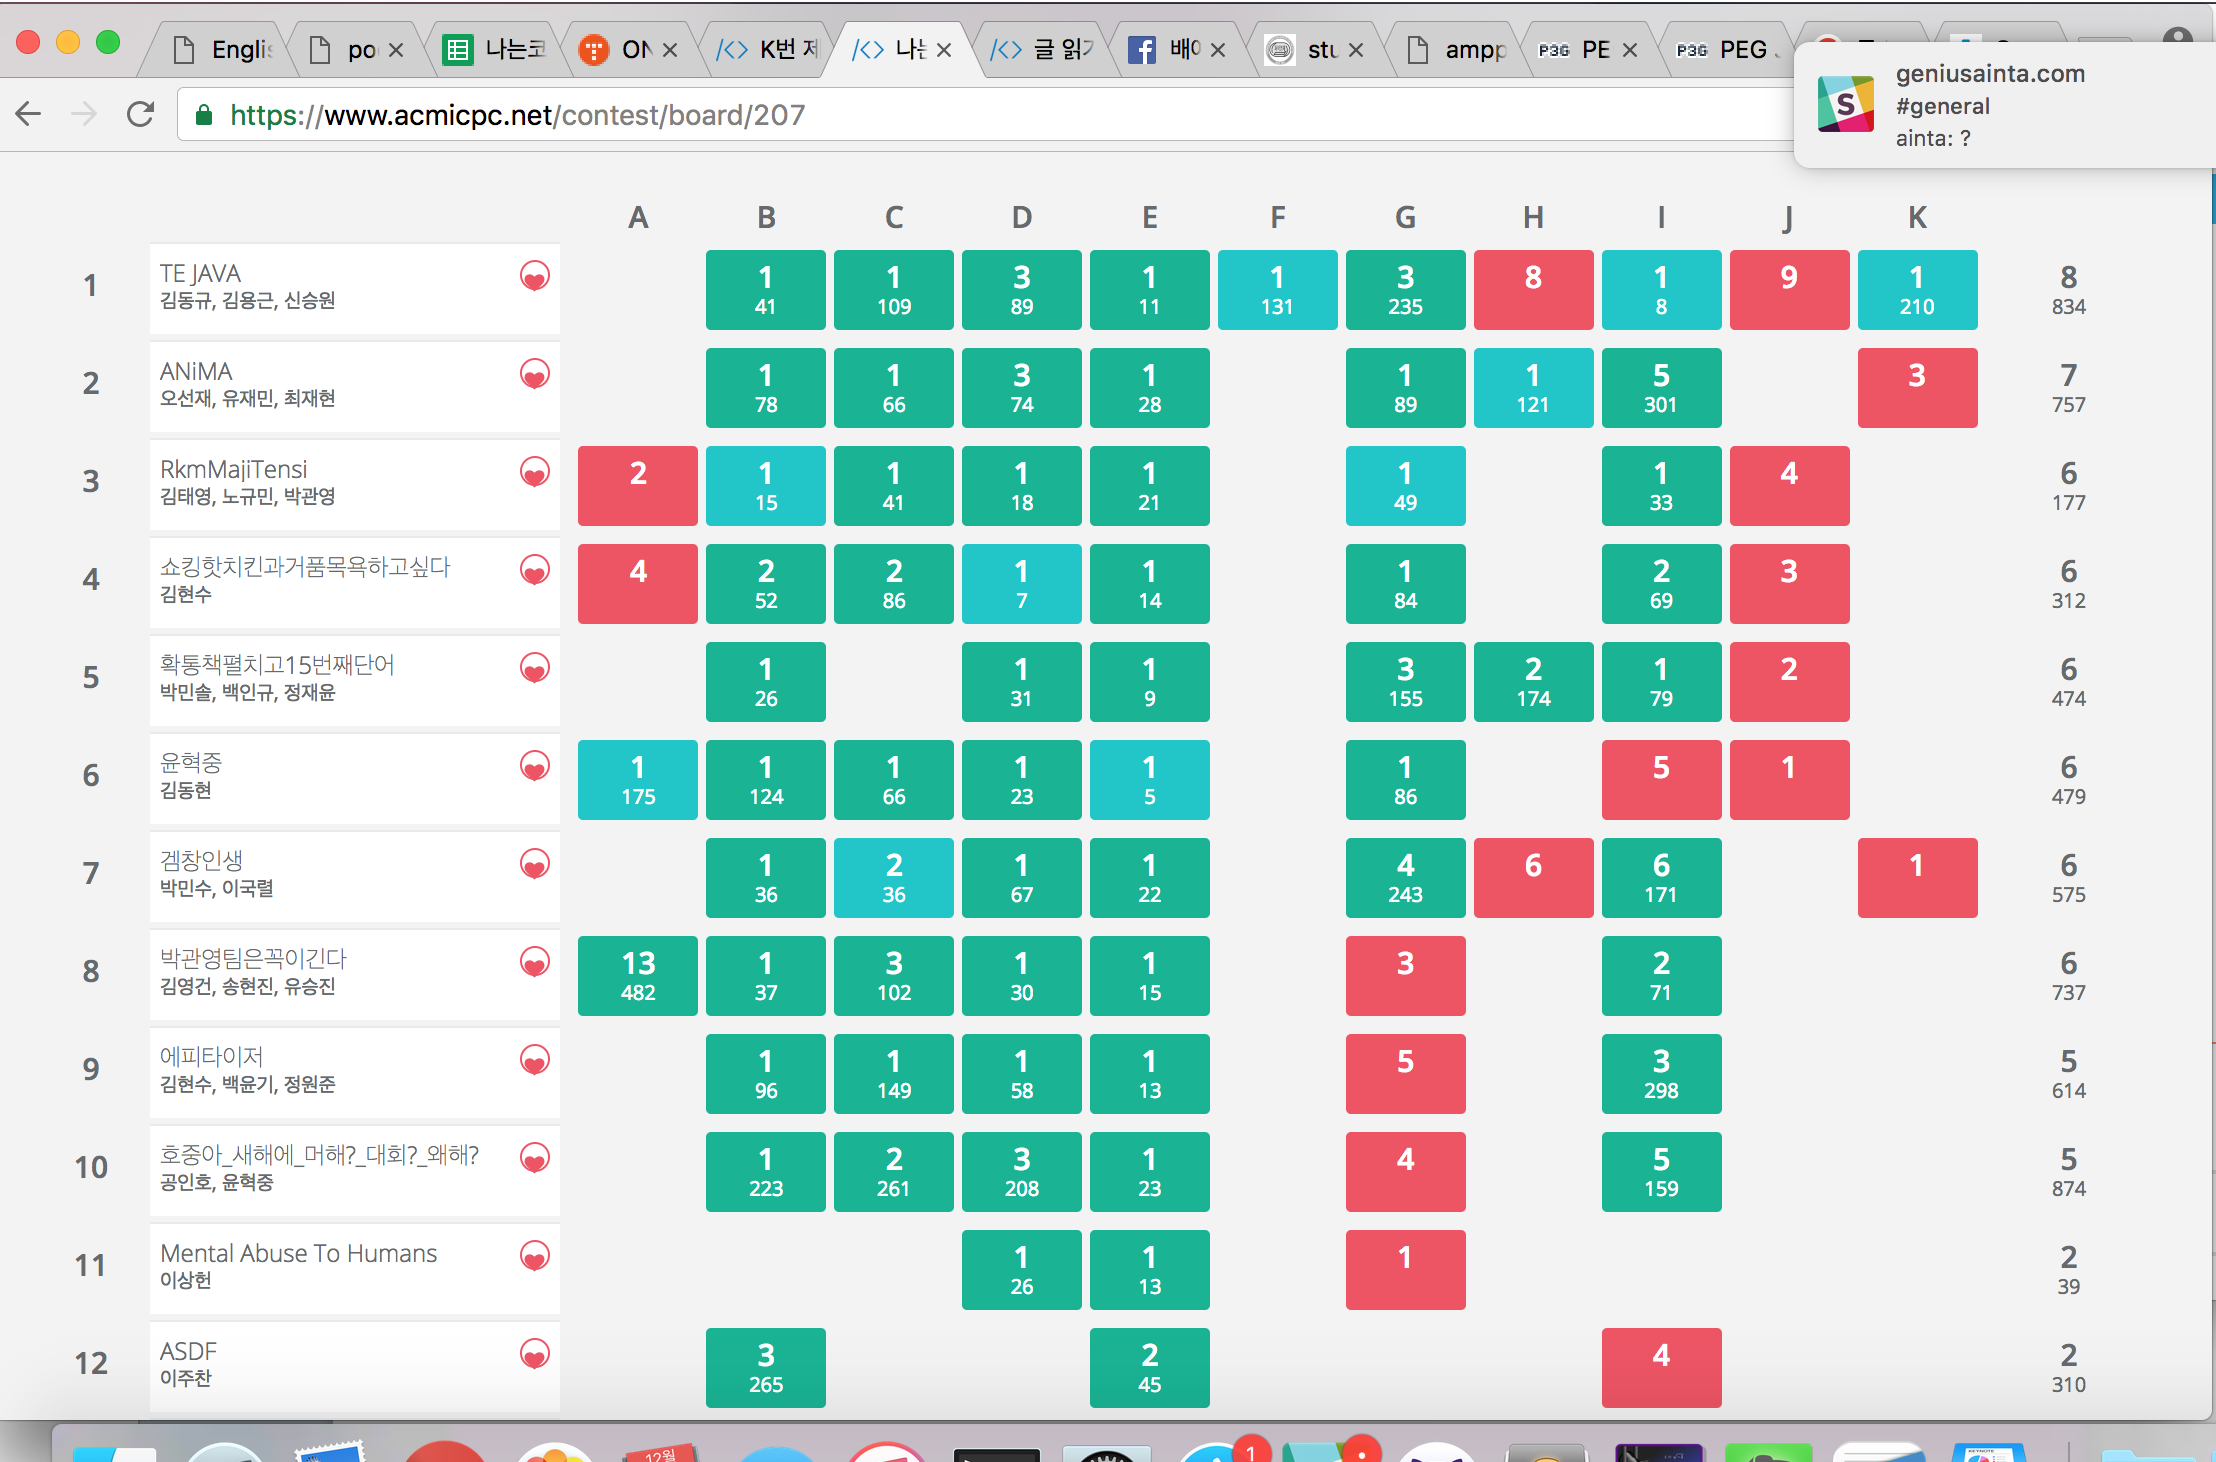
\includegraphics[scale=0.27]{IMG_2.png}
	\end{frame}

	\begin{frame}
(토요일날 참가해서 사진에 빠진 두명이 있습니다. ID tlwpdus님은 6/350 (6등), junis3님은 3/191 (10등).)
	\frametitle{Results : Open Contest 1}
	\begin{center}
		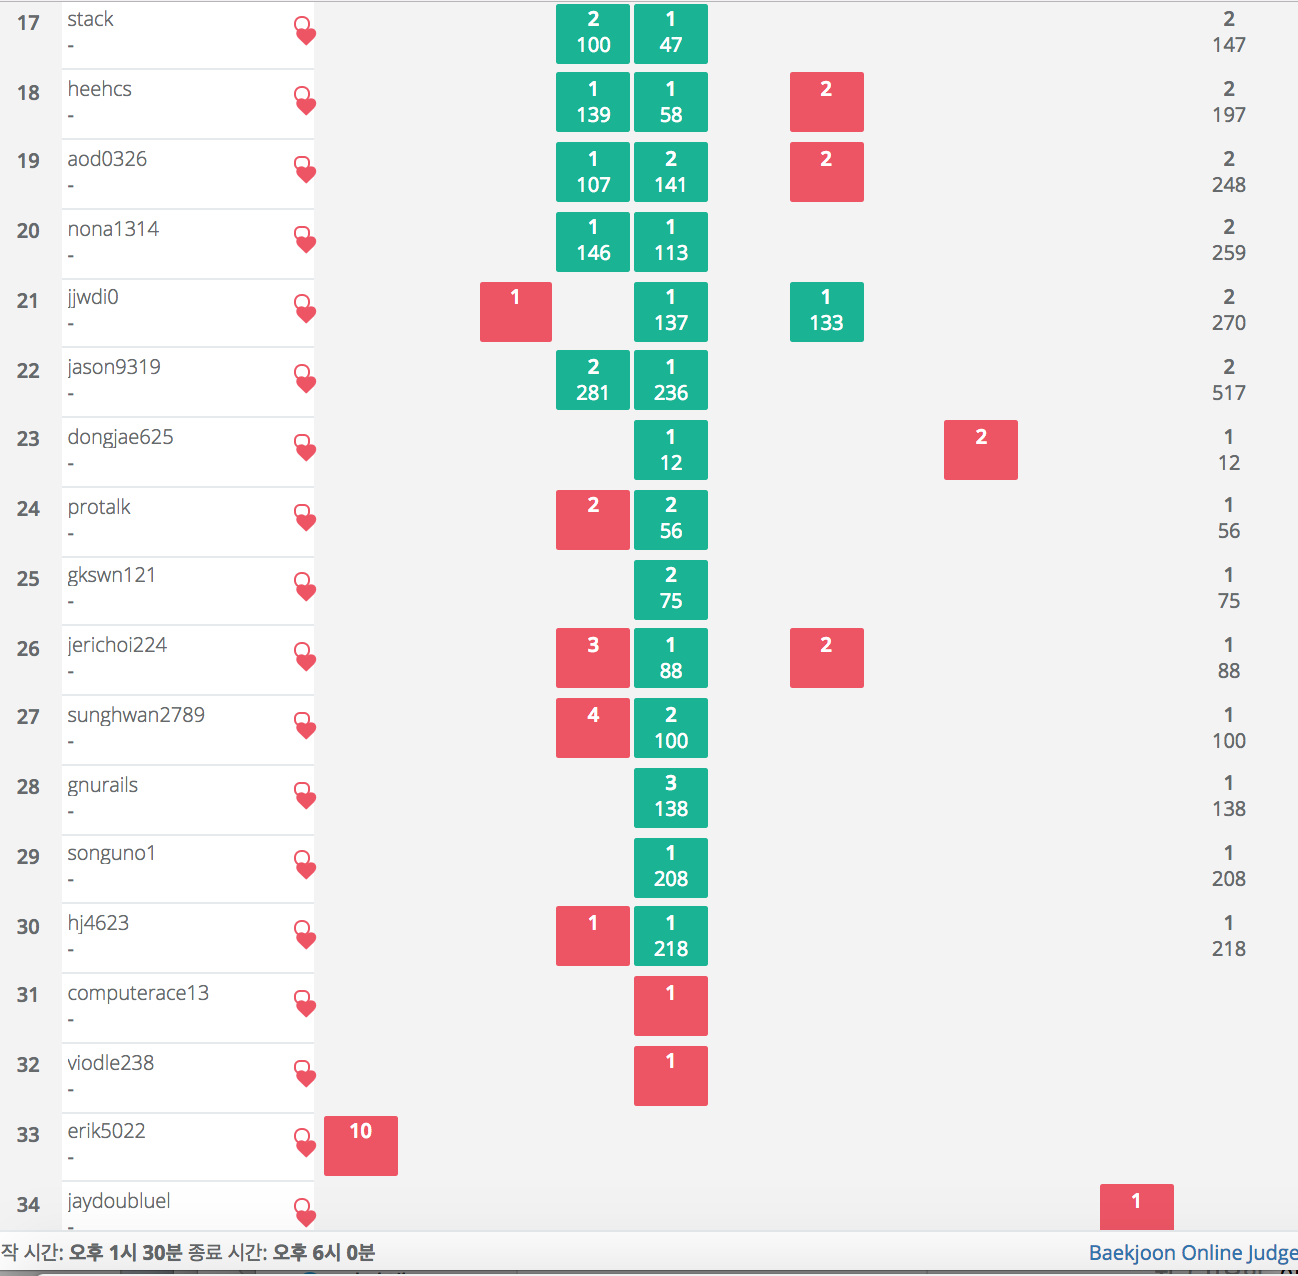
\includegraphics[scale=0.22]{IMG_3.png}
	\end{center}
\end{frame}

\begin{frame}
	\frametitle{Results : Open Contest 2}
	\begin{center}
		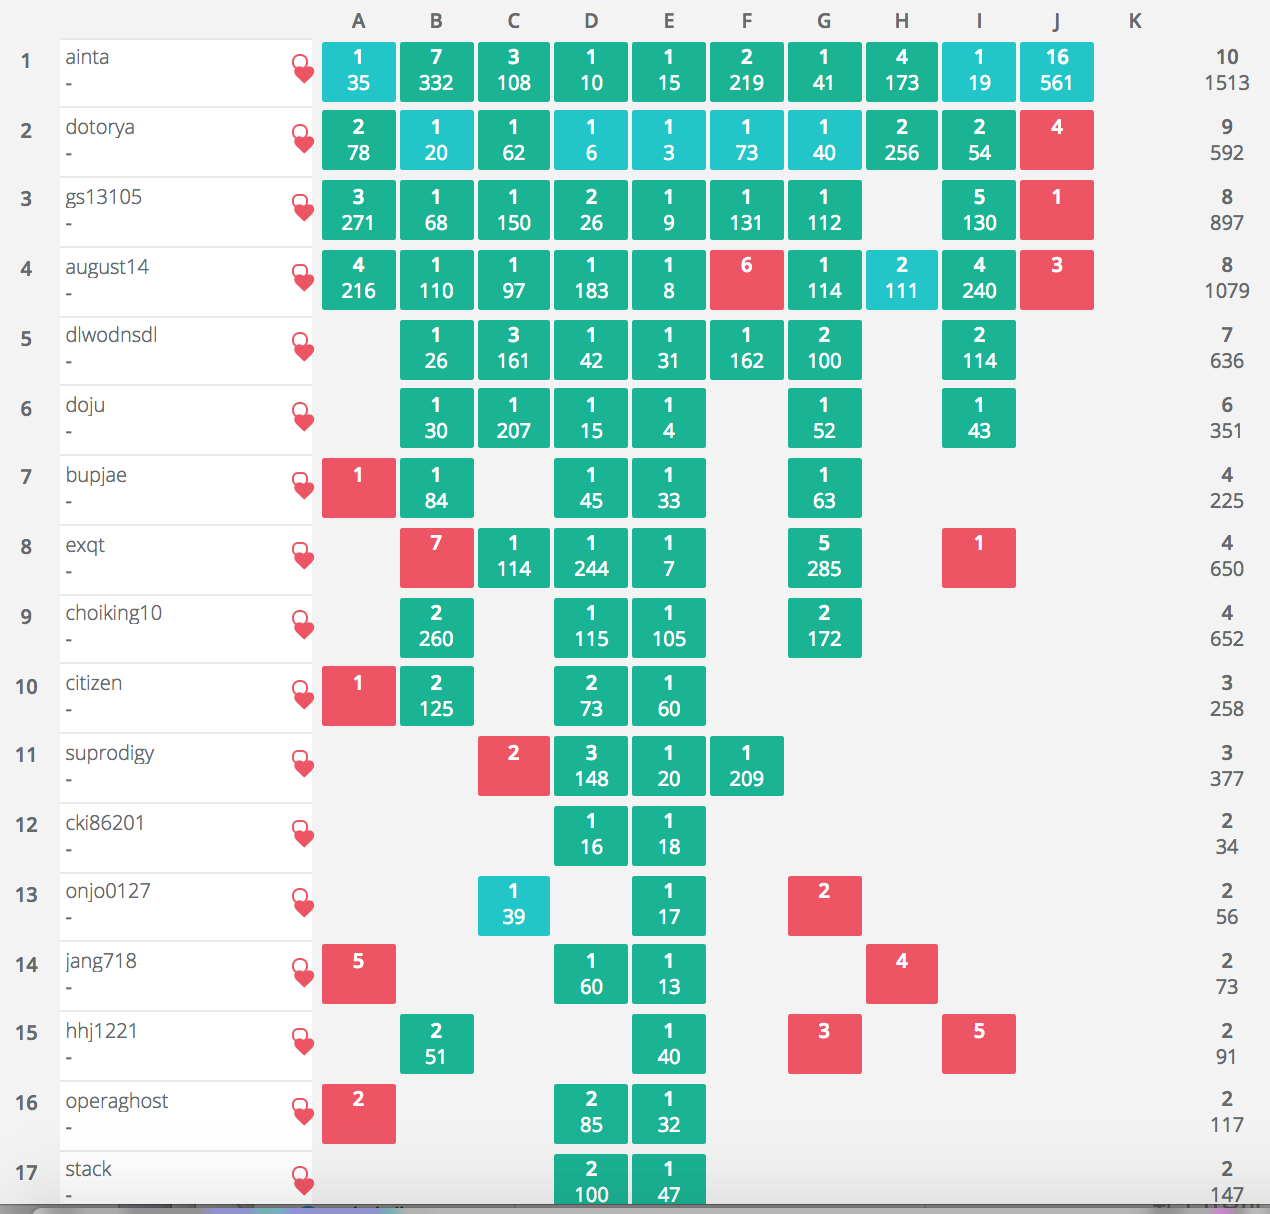
\includegraphics[scale=0.31]{IMG_4.png}
	\end{center}
\end{frame}

\begin{frame}
	\frametitle{Problem Statistics}
\begin{table}[]
	\centering
	\scalebox{0.85}{
	\label{my-label}
\begin{tabular}{|l|l|l|}
\hline
& 본선 정답자수 (12팀 참가)     & 오픈 정답자수 (36명 참가)  \\ \hline
A  & 2 (175min)        & 4 (35min)         \\ \hline
B  & 11 (15min)        & 12 (20min)        \\ \hline
C  & 9 (16min)         & 9 (39min)         \\ \hline
D  & 11 (7min)         & 21 (6min)         \\ \hline
E  & 12 (5min)         & 32 (3min)         \\ \hline
F  & 1 (131min)        & 5 (73min)         \\ \hline
G  & 7 (49min)         & 11 (40min)        \\ \hline
H  & 2 (121min)        & 3 (111min)        \\ \hline
I  & 9 (8min)          & 7 (19min)         \\ \hline
J  & 0                 & 1 (261min)        \\ \hline
K  & 1 (210min)        & 0                 \\ \hline
1등 & TE JAVA (8 / 834) & ainta (10 / 1513) \\ \hline
	\end{tabular}
}
\end{table}
\end{frame}

\begin{frame}
	\frametitle{A. 버스 여행}
	\begin{block}{$O((nm)^2)$ 알고리즘}
	 \begin{itemize}
		 	\item 관광 명소 각각의 격자상 위치를 $(x_i, y_i)$ 라 하고, 방문 시의 이득을 $c_i$, 건설 시기를 $a_i$ 라고 합시다.
		 	\item $a_i$ 순으로 정렬 후, 동적 계획법을 사용할 수 있습니다. $dp_i$ 를 $i$번 관광 명소를 방문했을 때의 이득이라 정의하면, 
		 	\item $dp_i = max_{a_j < a_i}(dp_j + |x_j - x_i| + |y_j - y_i|) + c_i$
	 \end{itemize}
 \end{block}
\end{frame}

\begin{frame}
	\frametitle{A. 버스 여행}
	\begin{block}{$O((nm)^2)$ 알고리즘}
		\begin{itemize}
			\item 관광 명소 각각의 격자상 위치를 $(x_i, y_i)$ 라 하고, 방문 시의 이득을 $c_i$, 건설 시기를 $a_i$ 라고 합시다.
			\item $a_i$ 순으로 정렬 후, 동적 계획법을 사용할 수 있습니다. $dp_i$ 를 $i$번 관광 명소를 방문했을 때의 이득이라 정의하면, 
			\item $dp_i = max_{a_j < a_i}(dp_j + |x_j - x_i| + |y_j - y_i|) + c_i$
		\end{itemize}
	\end{block}
	... 너무 느립니다. 어떻게 고쳐야 할까요?
\end{frame}
	
	
\begin{frame}
	\frametitle{A. 버스 여행}
		\begin{block}{분석 1}
		\begin{itemize}
			\item 일단 절댓값 식을 풀어봅시다. 4가지 케이스가 나옵니다. 
			\item $x_i \leq x_j$, $y_i \leq y_j$ 를 만족할 경우, $dp_i = max_{a_j < a_i}(dp_j + x_j - x_i + y_j - y_i) + c_i$ 라는 식이 나옵니다. 
			\item 풀어 쓰면 $dp_i = max_{a_j < a_i}(dp_j + x_j + y_j) - x_i - y_i + c_i$ 으로 정리됩니다.
			\item 나머지 케이스들도 거의 비슷한 식으로 전개 가능합니다. 
		\end{itemize}
	\end{block}
\end{frame}

\begin{frame}
\frametitle{A. 버스 여행}
		\begin{block}{분석 2}
\begin{itemize}
	\item 고로 $max_{a_j < a_i, x_i \leq x_j, y_i \leq y_j} (dp_j + x_j + y_j)$를 빠르게 구하면, 거기다가 $-x_i - y_i + c_i$ 만 더해주면 됩니다.
	\item 나머지 3개의 케이스도 똑같이 처리해주면 되니까, 저걸 빠르게 구하는 데 주목해 봅시다.
	\item $a_j < a_i$ 는 같은 $a_i$ 를 현명하게 계산하면 쉽게 처리할 수 있습니다. 설명은 패스.
	\item $x_i \leq x_j, y_i \leq y_j$ 가 어려워 보이네요. 그런데....
\end{itemize}
\end{block}
\end{frame}


\begin{frame}
	\frametitle{A. 버스 여행}
	\begin{block}{분석 3}
		\begin{itemize}
			\item 저 조건이 없이 순수히 $max_{j < i, a_j < a_i} (dp_j + x_j + y_j) - x_i - y_i + c_i$ 만 계산한다면, 어떤 문제가 생기나요?
			\item $x_i \leq x_j, y_i \leq y_j$ 일 때는 잘 구해지겠죠. 아닐 때는 계산한 식의 절댓값이 음수가 되어서 틀린 답이 될 겁니다.
		\end{itemize}
	\end{block}
\end{frame}

\begin{frame}
	\frametitle{A. 버스 여행}
	\begin{block}{분석 3}
		\begin{itemize}
			\item 저 조건이 없이 순수히 $max_{j < i, a_j < a_i} (dp_j + x_j + y_j) - x_i - y_i + c_i$ 만 계산한다면, 어떤 문제가 생기나요?
			\item $x_i \leq x_j, y_i \leq y_j$ 일 때는 잘 구해지겠죠. 아닐 때는 계산한 식의 절댓값이 음수가 되어서 틀린 답이 될 겁니다.
		\end{itemize}
	\end{block}
	\begin{block}{Key Observation}
		\begin{itemize}
			\item \textbf{그래도 상관 없습니다.} 절댓값이 음수가 되었다는 것은 원래 답보다 작은 답이 계산된다는 것입니다. 나머지 3개의 케이스를 처리하면서, 원래 답이 결국 반영됩니다.
		\end{itemize}
	\end{block}
\end{frame}

\begin{frame}
	\frametitle{A. 버스 여행}
	\begin{block}{$O(nmlg(nm))$으로의 개선}
		\begin{itemize}
			\item $max_{j < i, a_j < a_i} (dp_j + x_j + y_j)$ 는 변수 하나로 저장할 수 있습니다.
			\item 나머지 케이스도 각각 변수 하나로 저장할 수 있습니다.
			\item $dp_i$ 를 계산할 때, 4개의 케이스를 $O(1)$ 만에 처리할 수 있으며, 변수 역시 $O(1)$에 갱신할 수 있습니다. 고로 $dp$ 배열은 $O(nm)$에 채울 수 있습니다.
			\item 알고리즘의 최종 수행 시간은 $a_i$ 순으로 정렬하는 데 드는 $O(nmlg(nm))$ 입니다. AC.
		\end{itemize}
	\end{block}
\end{frame}
\begin{frame}
	\frametitle{A. 버스 여행}
	\begin{block}{$O(nmlg(nm))$으로의 개선}
		\begin{itemize}
			\item $max_{j < i, a_j < a_i} (dp_j + x_j + y_j)$ 는 변수 하나로 저장할 수 있습니다.
			\item 나머지 케이스도 각각 변수 하나로 저장할 수 있습니다.
			\item $dp_i$ 를 계산할 때, 4개의 케이스를 $O(1)$ 만에 처리할 수 있으며, 변수 역시 $O(1)$에 갱신할 수 있습니다. 고로 $dp$ 배열은 $O(nm)$에 채울 수 있습니다.
			\item 알고리즘의 최종 수행 시간은 $a_i$ 순으로 정렬하는 데 드는 $O(nmlg(nm))$ 입니다. AC.
			\item counting sort를 통해 $O(nm + max(a_i))$도 가능합니다.
		\end{itemize}
	\end{block}
\end{frame}
\begin{frame}
	\frametitle{A. 버스 여행}
	\begin{block}{$O(nmlg(n)lg(m))$}
		\begin{itemize}
			\item Key Observation을 안 해도 $O(nmlg(n)lg(m))$ 에 2D Segment Tree를 통해 구현할 수 있습니다. 자세한 설명은 생략합니다.
			\item Fenwick Tree스럽게 구현한 후 FastIO 를 쓰면 860ms 걸립니다. FastIO 안쓴 정해가 430ms라 그냥 막는 건 포기..
		\end{itemize}
	\end{block}
\end{frame}

\begin{frame}
	\frametitle{B. 큐브러버}
	\begin{block}{풀이 1}
		\begin{itemize}
			\item $N = 4$ 일 때, $x_1, x_2, x_3, x_4$ 를 알고 있으면 유일한 $a, b, c, d$를 항상 찾을 수 있습니다. 
			\item 고로, $N \leq 4$ 일 때는 항상 YES입니다. $N > 4$ 일 때는 찾은 $a, b, c, d$를 $x_5$ 부터 대입해서 식이 맞는지 검사하면 됩니다. 
			 \item 그래서 $a, b, c, d$ 를 어떻게 찾을까요? 
		\end{itemize}
	\end{block}
\end{frame}


\begin{frame}
	\frametitle{B. 큐브러버}
	\begin{block}{풀이 1}
		\begin{itemize}
			\item $N = 4$ 일 때, $x_1, x_2, x_3, x_4$ 를 알고 있으면 유일한 $a, b, c, d$를 항상 찾을 수 있습니다. 
			\item 고로, $N \leq 4$ 일 때는 항상 YES입니다. $N > 4$ 일 때는 찾은 $a, b, c, d$를 $x_5$ 부터 대입해서 식이 맞는지 검사하면 됩니다. 
			\item 그래서 $a, b, c, d$ 를 어떻게 찾을까요? $x_1 .. x_4$ 에 대해 쓰면 4개의 일차연립방정식이 나옵니다. 손으로 풀기는 번거로우니 울프람알파로 역행렬을 구해서 찾으면 됩니다. 
			\item 분수를 동반하지만 어쨌든 모든 계산은 정수 범위에서 가능합니다.
		\end{itemize}
	\end{block}
\end{frame}

\begin{frame}
	\frametitle{B. 큐브러버}
	\begin{block}{풀이 2}
		\begin{itemize}
			\item 모든 $1 \leq i \leq N$ 에 대해 $x_i = f_1(i)$인 3차 이하의 다항식 $f_1$가 존재한다는 것은, 
		\end{itemize}
	\end{block}
\end{frame}

\begin{frame}
	\frametitle{B. 큐브러버}
	\begin{block}{풀이 2}
		\begin{itemize}
			\item 모든 $1 \leq i \leq N$ 에 대해 $x_i = f_1(i)$인 3차 이하의 다항식 $f_1$가 존재한다는 것은, 
\item 모든 $2 \leq i \leq N$ 에 대해 $y_i = x_i - x_{i-1} = f_2(i)$인 2차 이하의 다항식 $f_2$가 존재한다는 것과 필요충분 관계이고,
		\end{itemize}
	\end{block}
\end{frame}

\begin{frame}
	\frametitle{B. 큐브러버}
	\begin{block}{풀이 2}
		\begin{itemize}			\item 모든 $1 \leq i \leq N$ 에 대해 $x_i = f_1(i)$인 3차 이하의 다항식 $f_1$가 존재한다는 것은, 
			\item 모든 $2 \leq i \leq N$ 에 대해 $y_i = x_i - x_{i-1} = f_2(i)$인 2차 이하의 다항식 $f_2$가 존재한다는 것과 필요충분 관계이고,
			\item 모든 $3 \leq i \leq N$ 에 대해 $z_i = y_i - y_{i-1}= f_3(i)$인 1차 이하의 다항식 $f_3$가 존재한다는 것과 필요충분 관계이고,
		\end{itemize}                                                                         
	\end{block}
\end{frame}


\begin{frame}
	\frametitle{B. 큐브러버}
	\begin{block}{풀이 2}
		\begin{itemize}
			\item 모든 $1 \leq i \leq N$ 에 대해 $x_i = f_1(i)$인 3차 이하의 다항식 $f_1$가 존재한다는 것은, 
\item 모든 $2 \leq i \leq N$ 에 대해 $y_i = x_i - x_{i-1} = f_2(i)$인 2차 이하의 다항식 $f_2$가 존재한다는 것과 필요충분 관계이고,
\item 모든 $3 \leq i \leq N$ 에 대해 $z_i = y_i - y_{i-1}= f_3(i)$인 1차 이하의 다항식 $f_3$가 존재한다는 것과 필요충분 관계이고,
\item 모든 $4 \leq i \leq N$ 에 대해 $w_i = z_i - z_{i-1} = f_4(i)$인 상수 함수..
		\end{itemize}
	\end{block}
\end{frame}


\begin{frame}
	\frametitle{B. 큐브러버}
	\begin{block}{풀이 2}
		\begin{itemize}
			\item 모든 $1 \leq i \leq N$ 에 대해 $x_i = f_1(i)$인 3차 이하의 다항식 $f_1$가 존재한다는 것은, 
\item 모든 $2 \leq i \leq N$ 에 대해 $y_i = x_i - x_{i-1} = f_2(i)$인 2차 이하의 다항식 $f_2$가 존재한다는 것과 필요충분 관계이고,
\item 모든 $3 \leq i \leq N$ 에 대해 $z_i = y_i - y_{i-1}= f_3(i)$인 1차 이하의 다항식 $f_3$가 존재한다는 것과 필요충분 관계이고,
\item 모든 $4 \leq i \leq N$ 에 대해 $w_i = z_i - z_{i-1} = f_4(i)$인 상수 함수..
			\item ????
		\end{itemize}
	\end{block}
\end{frame}


\begin{frame}
	\frametitle{B. 큐브러버}
	\begin{block}{풀이 2 (미분 아이디어)}
		\begin{itemize}
			\item 모든 $1 \leq i \leq N$ 에 대해 $x_i = f_1(i)$인 3차 이하의 다항식 $f_1$가 존재한다는 것은, 
			\item 모든 $2 \leq i \leq N$ 에 대해 $y_i = x_i - x_{i-1} = f_2(i)$인 2차 이하의 다항식 $f_2$가 존재한다는 것과 필요충분 관계이고,
			\item 모든 $3 \leq i \leq N$ 에 대해 $z_i = y_i - y_{i-1}= f_3(i)$인 1차 이하의 다항식 $f_3$가 존재한다는 것과 필요충분 관계이고,
			\item 모든 $4 \leq i \leq N$ 에 대해 $w_i = z_i - z_{i-1} = f_4(i)$인 상수 함수..
			\item ????
			\item PROFIT!
		\end{itemize}
	\end{block}
\end{frame}

\begin{frame}
	\frametitle{C. 크리스 마틴}
	\begin{block}{Greedy Solution}
		\begin{itemize}
			\item $A, C, G, T$ 중 가장 등장 수가 작은 알파벳을 찾아서, 그걸 $n$번 찍으면 풀 수 있습니다.
			\item 왜 될까요?

		\end{itemize}
	\end{block}
\end{frame}

\begin{frame}
	\frametitle{C. 크리스 마틴}
	\begin{block}{Greedy Solution}
		\begin{itemize}
			\item $A, C, G, T$ 중 가장 등장 수가 작은 알파벳을 찾아서, 그걸 $n$번 찍으면 풀 수 있습니다.
			\item 왜 될까요?
			\item 가장 등장 수가 작은 알파벳의 등장 수를 $F$라고 하고, 더 작은 답을 내는 문자열이 존재한다고 칩니다. 
			\item 이 문자열의 $A, C, G, T$의 개수는 모두 $F-1$ 이하여야 합니다. (아니면 그 알파벳만 찍는 공통 부분 수열이 존재)
			\item 다 합치면 길이가 $4F - 4$ 이하입니다. $F \leq n/4$ 라서 이러한 길이 $n$의 문자열은 존재하지 않습니다. 
		\end{itemize}
	\end{block}
\end{frame}

\begin{frame}
	\frametitle{D. 내일 할거야}
	\begin{block}{$O(nlgn)$ Greedy Solution}
		\begin{itemize}
			\item 보장이 되어 있다고는 하지만, 만약에 보장이 되어 있는지 없는지를 판별하는 문제를 푼다고 합니다. 어떻게 하나요?
			\item 현실에서 여러분들은 어떻게 하시나요? 저는 데드라인이 가장 빠른 것부터 하는데... 
		\end{itemize}
	\end{block}
\end{frame}
\begin{frame}
	\frametitle{D. 내일 할거야}
	\begin{block}{$O(nlgn)$ Greedy Solution}
		\begin{itemize}
			\item 보장이 되어 있다고는 하지만, 만약에 보장이 되어 있는지 없는지를 판별하는 문제를 푼다고 합니다. 어떻게 하나요?
			\item 현실에서 여러분들은 어떻게 하시나요? 저는 데드라인이 가장 빠른 것부터 하는데... 
			\item 네, 데드라인이 빠른 순으로 정렬해서, 그 순서대로 하는 것이 최적입니다. proof left as an exercise ㅎㅎ
		\end{itemize}
	\end{block}
\end{frame}

\begin{frame}
	\frametitle{D. 내일 할거야}
	\begin{block}{$O(nlgn)$ Greedy Solution}
		\begin{itemize}
			\item 초기에 노는 시간을 $T$만큼 확보한다는 것은, 데드라인을 모두 $T$ 만큼 감소시킨다는 것과 동치입니다. 
			\item 데드라인을 모두 일정하게 $T$만큼 감소시켜도, 데드라인의 대소 관계는 변하지 않습니다. 여전히 과제를 하는 가장 효율적인 방법은 데드라인이 빠른 순으로 진행하는 것입니다.
			\item 실제 얼마만큼의 노는 시간을 확보할 수 있는지는, 실제 배정 순의 역순으로 시간을 계산해나가면서 가능합니다. 아니면, Parametric Search를 사용해도 됩니다. 
		\end{itemize}
	\end{block}
\end{frame}

\begin{frame}
	\frametitle{E. 풍선 놀이}
	\begin{block}{Do you know C++?}
		\begin{itemize}
			\item 풍선이 설치되었는지 아닌지를 배열로 관리합니다.
			\item 반복문으로 풍선을 설치합니다. 
			\item \lstinline[language=C++,basicstyle=\ttfamily]{for(int j=l; j<=n; j+=i) chk[j] = 1;}
			\item 최후에 배열을 전부 돌면서 \lstinline[language=C++,basicstyle=\ttfamily]{chk[i] == 0}인 원소를 셉니다.
			\item 꿀팁 : 	\lstinline[language=C++,basicstyle=\ttfamily]{cout << count(chk+1, chk+n+1, 0);}
			
		\end{itemize}
	
	\end{block}
\end{frame}



\begin{frame}
	\frametitle{F. 장비를 정지합니다}
	\begin{block}{$O(n+m)$ 알고리즘 1}
		\begin{itemize}
			\item DFS를 통해 DP를 구현해 봅시다. $mincost(i)$ = i번 정점의 장비를 정지하는 최소 비용 이라고 정의합시다. 
			\item 강한 충격을 주면 $z_i$만큼 쓰면 되고, 약한 충격일 때는 $u_i$ + $\sum_{j \in g_i} mincost(j)$의 비용이 듭니다. 정의는 쉽습니다. 
			\item 하지만, 이대로 짜면 예제도 안나옵니다. 무한루프...
		\end{itemize}
		
	\end{block}
\end{frame}

\begin{frame}
	\frametitle{F. 장비를 정지합니다}
	\begin{block}{$O(n+m)$ 알고리즘 2}
		\begin{itemize}
			\item 무한 루프가 걸리는 이유는, $mincost(i)$ 를 계산하기 위해 $mincost(i)$ 를 호출하는 일이 생기기 때문입니다. 생각해보면, 이러한 형태로는 최적화가 되지 않기 때문에 쓸모가 없습니다. 
			\item 고로 이러한 경우를 없애기 위해서, 현재 계산중인 (계산이 이뤄지지 않은, 아주 끝난것도 아닌, 계산 중인) 정점을 호출했을 때는 더 진행하지 않고 $\infty$ 를 반환합니다. 
			\item 재귀 stack에 있는 원소를 체크하는 식으로 할 수 있습니다.
			\item 시간 복잡도는 $O(n+m)$ 입니다.
		\end{itemize}
	\end{block}
\end{frame}

\begin{frame}
	\frametitle{G. 순열 그래프의 연결성 판별}
	\begin{block}{$O(n)$ 풀이}
		\begin{itemize}
			\item $i$ 까지의 연결성을 결정했을 때, 이를 토대로 $i+1$까지의 연결성을 결정해 봅시다.
			\item 각각의 컴포넌트는 순열 상에서 연결된 구간의 형태 ($s, s+1, s+2, ..., e$) 를 띕니다. 스택에 각각의 컴포넌트를 번호 순으로 저장합니다.
			\item 현재 정점을 유일한 원소로 갖는 컴포넌트를 만듭니다. 
			\item 현재 들어간 정점이 스택의 top에 있는 컴포넌트에 속한다면, 현재 컴포넌트에 스택의 top에 있는 컴포넌트를 합쳐줍니다. 그렇지 않다면 현재 컴포넌트를 스택에 넣습니다.  
		\end{itemize}
	\end{block}
\end{frame}

\begin{frame}
	\frametitle{G. 순열 그래프의 연결성 판별}
	\begin{block}{$O(n)$ 풀이}
		\begin{itemize}
			\item 그럴듯 하지만, 그냥 짜면 왠지 $O(n^2)$ 가 나올 것 같은 풀이입니다.
			\item 이를 타개하기 위해서 스택에 컴포넌트를 조금 더 현명하게 넣어야 합니다. 각각의 컴포넌트에 4개의 정보를 부여합시다 : 구간의 시작점, 끝점, 구간 $a_i$ 최대, 최소.
			\item 이 4가지 값을 통해서 위에 제시한 연산을 모두 $O(n)$에 할 수 있습니다. 
			\item $n$ 개의 연결성을 모두 파악했다면 print만 해주면 됩니다.
		\end{itemize}
	\end{block}
\end{frame}

\begin{frame}
	\frametitle{G. 순열 그래프의 연결성 판별}
	\begin{block}{$O(n)$ 풀이 2}
		\begin{itemize}
			\item 순열 그래프의 컴포넌트는 연속한 구간으로 쪼개져 있다고 말했습니다.
			\item 그렇다면, 어떠한 상황에 구간이 쪼개질까요?
			\item $[1, i]$ 구간의 $a_i$ 최댓값이 $i$인 것과 구간이 $[?, i]$ 와 $[i+1, ?]$ 으로 쪼개지는 것이 동치입니다.
			\item 고로 쉽게 $O(n)$에 풀 수 있습니다. 
		\end{itemize}
	\end{block}
\end{frame}

\begin{frame}
	\frametitle{H. 두더지 잡기}
	\begin{block}{$O(nk)$ 동적 계획법}
		\begin{itemize}
			\item 한번 두더지를 쫓아낸 곳에 또 다시 두더지를 쫓을 이유는 없습니다. (굳이 상황을 만들 수는 있지만 매우 비효율적...)
			\item 원호에다가 두더지가 도망간 곳을 다 마킹했다고 쳐 봅시다.
			\item 당연하지만 마킹된 곳에 있는 두더지는 다 도망갑니다.
			\item 인접한 두 마킹된 위치가 거리 3 이상이라면, 그 사이에 있는 두더지는 도망가지 않습니다.
			\item 인접한 두 마킹된 위치가 거리 2 이하면, 그 사이에 있는 두더지를 도망가게 할 수 있습니다.
			\item OVOOVOVVOVOOV $\rightarrow$ XXOOXXXXXXOOX
		\end{itemize}
	\end{block}
\end{frame}

\begin{frame}
	\frametitle{H. 두더지 잡기}
	\begin{block}{$O(nk)$ 동적 계획법}
		\begin{itemize}
			\item 결론적으로, 두 쫓아낸 위치 사이에 있는 두더지들은 모두 도망갑니다. 
			\item 원을 직선으로 폈다면, $O(nk)$ 에 문제를 해결할 수 있습니다. $dp_{i, j}$ = $i$ 번 지점까지 총으로 $j$번 쫓아냈을 경우라고 정의하면 됩니다.
			\item 하지만 직선으로 펼 수 없죠... 원호에서는 이를 적당히 처리하셔야 합니다. 
			\item 이 부분은 알고리즘적으로 어렵지는 않고 구현이 힘듭니다. 
		\end{itemize}
	\end{block}
\end{frame}

\begin{frame}
	\frametitle{H. 두더지 잡기}
	\begin{block}{$O(nk)$ 동적 계획법}
		\begin{itemize}
			\item 결론적으로, 두 쫓아낸 위치 사이에 있는 두더지들은 모두 도망갑니다. 
			\item 원을 직선으로 폈다면, $O(nk)$ 에 문제를 해결할 수 있습니다. $dp_{i, j}$ = $i$ 번 지점까지 총으로 $j$번 쫓아냈을 경우라고 정의하면 됩니다.
			\item 하지만 직선으로 펼 수 없죠... 원호에서는 이를 적당히 처리하셔야 합니다. 
			\item 이 부분은 알고리즘적으로 어렵지는 않고 구현이 힘듭니다. 
			\item 그래서 Left as an exercise ㅎㅎㅎ	
	\end{itemize}
	\end{block}
\end{frame}


\begin{frame}
	\frametitle{I. 수열}
	\begin{block}{$O(n)$ 동적 계획법}
		\begin{itemize}
			\item 홀수냐 짝수냐만이 중요합니다. 고로 홀짝성을 적절히 결정해서 주어진 식을 만족시켜야 합니다. 
			\item 모든 $1 \leq i \leq n-k$ 에 대해서, $a_i + a_{i+1} + ... + a_{i+k-1} \equiv a_{i+1} + ... + a_{i+k-1} + a_{i+k}\ (mod\ 2)$ 입니다. 
			\item 양변을 정리하면 모든 $1 \leq i \leq n-k$ 에 대해서, $a_i  \equiv a_{i+k}\ (mod\ 2)$ 입니다.
			\item 이 때문에, $a_1, ..., a_k$ 의 홀짝성을 정해주면 그 이후 원소의 홀짝성은 자동으로 결정됩니다. 
		\end{itemize}
	\end{block}
\end{frame}



\begin{frame}
	\frametitle{I. 수열}
	\begin{block}{$O(n)$ 동적 계획법}
		\begin{itemize}
			\item $a_1 + a_2 + ... + a_k \equiv 0\ (mod\ 2)$ 입니다.
			\item 이걸 만족하면 나머지 식은 다 만족이 됩니다.
			\item $a_i$ 를 짝수로 만들면, $a_i, a_{i+k}, a_{i+2k} .. $ 중 홀수인 애들은 전부 바꿔줘야 합니다. 이런 개수를 다 세줍시다.
			\item 이제 $dp_{i, j} =$ $i$번 원소까지의 합이 $j\ (mod\ 2)$ 인 경우의 수 라고 정의하고 풀면, $O(n)$ 에 해결 가능합니다. 
		\end{itemize}
	\end{block}
\end{frame}

\begin{frame}
	\frametitle{J. 비무장 지대}
	\begin{block}{관찰 1}
		\begin{itemize}
			\item 각각의 지뢰를 터트렸을 때, 연속적인 지뢰 폭발이 일어날 것입니다. 이러한 연속적인 폭발로 파괴되는 지역은 하나의 연속된 구간을 이룹니다.
			\item 이걸 $PL_i, PR_i$ 와 같이 어떻게 계산했다고 쳐봅시다. 이후에는 정렬 후 간단한 sweeping을 하면 오프라인으로 $O((n+m)lg(n+m))$에 풀 수 있습니다.
			\item 핵심은 $PL_i, PR_i$ 를 빠르게 계산하는 겁니다.
		\end{itemize}
	\end{block}
\end{frame}

\begin{frame}
	\frametitle{J. 비무장 지대}
	\begin{block}{관찰 2}
		\begin{itemize}
			\item 여기서 아주 다양한 풀이가 있을 것이라고 생각합니다. 제 풀이는 다음과 같습니다.
			\item 편의상 $PL_i$ 만 구하다고 하겠습니다. $PR_i$ 는 반대로 뒤집어서 똑같이 계산 가능합니다.
			\item $PL_i$ 는 어떠한 지뢰의 $L_i$ 값 중 하나일 겁니다. 각각의 지뢰를 $L_i$ 순으로 정렬해서, Flood Fill의 요령으로 거꾸로 $PL_i$ 에 칠해봅시다. 
			\item 단순하게 하면 $O(n^2)$니까, $O(nlgn)$ 으로 줄여봅시다. 
		\end{itemize}
	\end{block}
\end{frame}


\begin{frame}
	\frametitle{J. 비무장 지대}
	\begin{block}{관찰 3}
		\begin{itemize}
			\item 거꾸로 하는 거니까, 현재 지뢰를 터트릴 수 있는 지뢰의 조건을 생각해 봅시다. $X_j - L_j <= X_i$ 이며, $X_j + R_j >= X_i$ 인 지뢰 $j$ 는 $i$에서 도달 가능합니다.
			\item 자료 구조를 생각해 봅시다. 일단 저러한 지뢰 하나를 방문하기만 하면, 다시 방문할 필요가 없습니다. $O(lgn)$ 시간 안에 저러한 지뢰 하나를 반환하고, 지울 수 있다면...
			\item \textbf{Segment Tree를 사용합시다!} $X_j - L_j$ 를 인덱스로 하고, $X_j + R_j$ 를 값으로 하는 Maximum Segment Tree를 사용합니다. 
		\end{itemize}
	\end{block}
\end{frame}


\begin{frame}
	\frametitle{J. 비무장 지대}
	\begin{block}{$O(nlgn)$ 풀이}
		\begin{itemize}
			\item $X_j - L_j$ 이하의 구간에서, $X_j + R_j$ 값을 최대로 하는 지뢰 하나가 만약에 도달 불가능하다면, 그 상황에서 종료합니다.
			\item 그렇지 않다면, 그 지뢰를 제거한 후 방문합니다. 
			\item 지뢰를 지우는 것은 원소 갱신으로 대체 가능합니다.
			\item 좌표 범위가 큰 것은 적당한 좌표 압축으로 해결합시다.
		\end{itemize}
	\end{block}
\end{frame}


\begin{frame}
	\frametitle{J. 비무장 지대}
	\begin{block}{연습 문제}
		\begin{itemize}
			\item 이런 식으로 특수한 그래프에서 DFS를 빠르게 하는 유형의 문제들이 몇개 있습니다. 굳이 정해가 아니더라도 굉장히 여러 문제의 풀이에 도움이 돼요.
			\item Can of Worms: \url{https://www.acmicpc.net/problem/7149}
			\item 전선 연결하기: \url{https://www.acmicpc.net/problem/11915/}
		\end{itemize}
	\end{block}
\end{frame}

\begin{frame}
	\frametitle{K. 그래프와 쿼리}
	\begin{block}{DP + 이진 탐색 $O(nm + qlgn)$}
		\begin{itemize}
			\item 풀이가 두개 있습니다. 이건 제가 풀었던 방법입니다. 
			\item 쿼리를 오프라인으로 처리해 봅시다. 간선을 끊는 대신, 각각의 간선에 가중치 $t_i$ 를 매겨봅시다. 
			\item 간선이 끝까지 끊기지 않는다면 $t_i = \infty$ 이고, 끊긴다면 그 쿼리가 들어온 시점을 $t_i$ 에 저장합니다.
			\item 어떠한 경로가 쿼리 시점 $T$에 사용 가능하려면, 그 경로 상에 있는 모든 간선이 $t_i > T$ 를 만족해야 합니다.
		\end{itemize}
	\end{block}
\end{frame}

\begin{frame}
	\frametitle{K. 그래프와 쿼리}
	\begin{block}{DP + 이진 탐색 $O(nm + qlgn)$}
		\begin{itemize}
			\item 이제 DP를 합시다. DP 정의는 벨만 포드와 유사합니다.
			\item $dp_{i, j} = $ 1 - $j$를 잇는 모든 길이 $i$ 이하의 경로 중, $t$의 최솟값을 최대화하는 경로의 $t$ 값.
			\item $O(nm)$ 에 계산 가능합니다.
			\item 이제, E 쿼리를 처리합니다. $dp_{dist, p} > i$ 를 만족하는 최소의 $dist$ 가 E 쿼리의 답입니다.
			\item 이는 이진 탐색으로 $O(qlgn)$ 에 찾을 수 있으며, 사실 $O(qn)$ 에 찾아도 엄청 빠르게 나옵니다.
		\end{itemize}
	\end{block}
\end{frame}
\begin{frame}
	\frametitle{K. 그래프와 쿼리}
	\begin{block}{다른 풀이}
		\begin{itemize}
			\item TE JAVA 팀과 박범수 (IOI 2012 금메달리스트) 님이 이렇게 푸셨습니다.
			\item 쿼리를 거꾸로 처리해서, 간선을 더해주는 형태로 처리합니다. 처음에 BFS로 최단 거리를 다 저장합니다.
			\item 간선이 추가되면 최단 거리가 줄어들기도 합니다. 이 때 줄어드는 모든 경우에 대해서 BFS로 naive하게 뿌려줍니다.
			\item naive하게 뿌려줬으니 $O(qm)$ 이라고 생각할 수 있겠지만, 뿌려주는 경우에 대해서는 거리가 항상 감소하거나, 도달 불가능한 정점이 도달 가능해 집니다. 각각의 정점을 방문하는 횟수는 많아야 $O(n)$번이라, 시간 복잡도는 $O(nm + q)$ 입니다. 
		\end{itemize}
	\end{block}
\end{frame}
\end{document}
